\section{Controlled Texture Experiments}
\label{sec:textures}
\subsection{Protocol and numerical checks}
We generate $32\times32$ periodic textures using four directions, two radial bands per direction, and two independent conjugate frequency pairs per group, for $d=16$ independent power coordinates. The initial spectrum is flat. Images remain floating point without per-image normalization or clipping. Pretraining uses no downstream labels. Ten predefined unit-variance tasks comprise two individual power coordinates and eight direction/band energy sums; all are evaluated on the same checkpoints.

The main bottleneck has $C=8$, $K=1$; extensions use $K=2$ or $11\times11$ periodic kernels. Parameters have no bias, batch normalization, weight decay, momentum, or output normalization. We compare $r=\eta_W/\eta_h\in\{0.1,1,10\}$. Each seed shares initial effective representations and paired data/augmentation streams across ratios. Controls are direct effective-map optimization, ordinary linear factorization on the same $q$, and frozen layers. A linear control on raw pixels would change task expressivity and is not used.

We retain two calibration protocols. The matched-parameter protocol starts from the same $B_0,W_0$. Independent calibration instead uses each model's parameter Jacobian Gram traces, without task labels, to equalize its two active blocks and normalize initial total mobility. Scalar factor rescaling preserves $A_0$ and encoder row space. Equal traces do not imply equal update directions. Development seeds 0 and 1 are separate from ten confirmation seeds 2--11. Population protocols were locked before confirmation; settings reuse the same ten seeds and do not supply independent repetitions.

Spatial convolution, FFT evaluation, and effective-map gradients are checked independently. Centered spatial output agrees with $Aq$ to approximately $9.71\times10^{-17}$, and the spatial/FFT gradient discrepancy is approximately $6.94\times10^{-18}$. The real-parameter fixed-section error at $\ell=6$ decreases from approximately $4.02\times10^{-4}$ to $2.01\times10^{-4}$ when the step is halved. An independent empirical gradient check has approximately $1.98\%$ relative error, reflecting moment estimation rather than machine-precision equivalence. No finite-sample trajectory is treated as a pointwise theorem reproduction.

\subsection{Population subspace selection}
The confirmation suite contains three architectures, two calibrations, three models, three ratios, and ten paired seeds: 540 population trajectories. Its primary comparison is the common section $\ell=3$. Let $D_X=\norm{P_{X(t)}-P_{X(0)}}_F$. Table~\ref{tab:population} reports independently calibrated $r=1$ means.

\begin{table}[t]
\centering\small
\caption{Population subspace displacement at $\ell=3$, independently calibrated $r=1$, ten paired seeds. Linear encoder conservation coexists with projection motion.}
\label{tab:population}
\setlength{\tabcolsep}{3pt}
\begin{tabular}{lrrrr}
\toprule
&\multicolumn{2}{c}{Encoder $D_B$}&\multicolumn{2}{c}{Projection $D_A$}\\
Setting&Square&Linear&Square&Linear\\\midrule
$K=1$, full&0.3064&$1.15\,10^{-14}$&0.5161&0.6087\\
$K=2$, full&0.4499&$1.23\,10^{-14}$&0.5597&0.5319\\
$K=1$, local&0.3786&$1.26\,10^{-14}$&0.5572&0.6196\\
\bottomrule
\end{tabular}
\end{table}

Every observed square-model seed has resolvable encoder motion, whereas linear encoder displacement remains at rounding scale. Frozen-front displacement is zero. All observed encoder and projection ranks remain $8$ and $K$. Changing $r$ also changes square-model displacement: for $K=1$ full support, its mean is $0.7161$, $0.3064$, and $0.0485$ for the three ratios. These are geometric changes, not uniformly worse task risks. Direct optimization of a scalar effective map under the radial population objective preserves its direction, while ordinary linear factorization can change projection risk. Rebound is therefore not unique to the square architecture.

\subsection{Complete empirical training and reproducible drift}
We train from initialization on 32,768 unlabeled images, batch size 256, for 4,000 updates. Full-support and local-kernel suites each contain 90 trajectories: three models, three ratios, and ten seeds. All reach the prespecified common section $\ell=1.5$. Forty additional trajectories provide three independent SGD streams per seed for the square and linear models at the repeated condition. Table~\ref{tab:empirical} reports encoder displacement.

\begin{table}[t]
\centering\small
\caption{Encoder displacement after complete empirical training, evaluated at common $\ell=1.5$; ten-seed means. Frozen-front values are zero.}
\label{tab:empirical}
\begin{tabular}{llrrr}
\toprule
Kernel&Model&$r=0.1$&$r=1$&$r=10$\\\midrule
Full&Square&0.41312&0.13692&0.01843\\
Full&Linear&0.02336&0.00666&0.00089\\
Local&Square&0.44250&0.17740&0.02626\\
Local&Linear&0.02851&0.00920&0.00123\\
\bottomrule
\end{tabular}
\end{table}

Empirical square-model geometry remains close to the corresponding population state: at $r=1$, $\ell=1.5$, the empirical/population encoder projector distance averages $0.00713$ for full support and $0.00850$ for local kernels, compared with movements of $0.13692$ and $0.17740$ from initialization. This agreement concerns this model family, dataset size, and training budget.

Linear encoder movement is nonzero and reproducible. Conditional on initialization and the finite dataset, the mean pairwise cosine between terminal projector changes from independent streams is $0.9810$ for the square model and $0.8683$ for the linear model. These are within-seed agreements, not evidence for a universal direction across initializations. Finite datasets need not have isotropic power covariance, so their conditional expected gradient need not satisfy Proposition~\ref{prop:linear}. Exploratory conditional-moment calculations on two development states support this explanation. Nonlinear sample-moment estimation and finite update size may also contribute; the diagnostic is not an independently confirmed decomposition of all drift.

\begin{figure}[t]
\centering
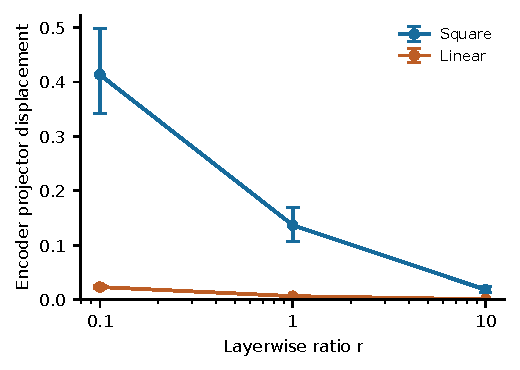
\includegraphics[width=\linewidth]{figures/empirical_subspaces.pdf}
\caption{Full-support empirical encoder displacement at common $\ell=1.5$. Error bars are descriptive paired-seed bootstrap intervals from the saved summary. Square-model motion is larger, but finite-data linear motion is nonzero.}
\label{fig:empirical}
\end{figure}

\subsection{Intervention prediction has a training-stage boundary}
The final test uses checkpoints at updates 500, 2,000, and 3,500 from complete empirical training. Each of 90 model/seed/checkpoint states has 32 independent future batch/augmentation streams. At the midpoint, eight streams continue for 8 and 64 updates. Population geometry predicts task-conditioned risk changes before drawing future batches; actual branches use empirical GUPA updates. Seed averages, rather than branches or tasks, determine summaries.

For the square model, single-step sign agreement is $91.8\%$, $57.0\%$, and $52.6\%$ at the three stages; constant-decrease baselines are $55.6\%$, $47.7\%$, and $50.8\%$. At the midpoint the sign of the repeated-batch mean agrees $92.3\%$ of the time even though individual batches agree only $57.0\%$. Late agreement is close to baseline for both summaries. This distinguishes prediction of an average direction from reliable control of a single stochastic update.

Longer midpoint windows raise sign agreement to $69.8\%$ and $71.0\%$, but amplitude mean absolute error rises from approximately $1.2\times10^{-5}$ for one update to $6.7\times10^{-4}$ for 64 updates. Noise averaging can improve signs while the first-order magnitude approximation worsens. For the prespecified primary task, positive population thresholds occur in 5/10 early states and only 1/10 at each later stage. Threshold errors are reported only where comparable positive thresholds exist; we do not force every state to admit a reversal. The intervention remains an oracle mechanism experiment using known $\beta$.

\begin{figure}[t]
\centering
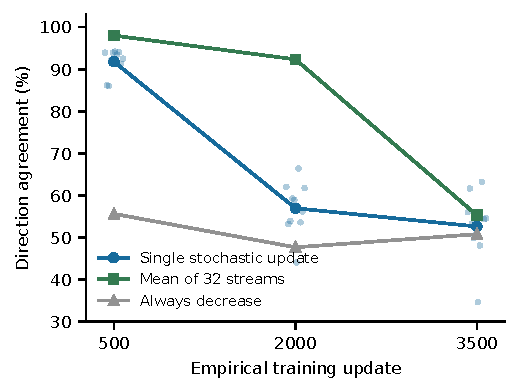
\includegraphics[width=\linewidth]{figures/intervention_boundary.pdf}
\caption{Square-model one-update direction predictions at empirical checkpoints. Markers average ten seed-level summaries; thin points show seeds. The distinction between individual stochastic updates and replicate means disappears late.}
\label{fig:intervention}
\end{figure}

\subsection{Frozen-source predictions on independent future streams}
\label{sec:texture-motion-prediction}
A separate protocol calibrates the actual finite-batch field at saved checkpoints and freezes all predictions before drawing future streams. Development uses seeds 0--1 at updates 500 and 2,000 (12 states); validation uses seeds 2--11 at updates 500, 2,000, and 3,500 (90 states). Each includes square, linear, and frozen-front models. These are held out from tuning this protocol, not previously unseen training runs in every earlier analysis. All planned states completed without rank failures. At each source, 16 fit batches, 32 error batches, and four eight-step probe streams precede eight independent validation streams. The three ratios share paired randomness. The ten predefined tasks and source-constructed competitors are reported separately.

The prediction is the frozen source task slope times the horizon. Inflated calibration quantiles give empirical intervals, not uniform stochastic certificates. The usable horizon is at most eight by the declared probe support; zero reported coverage at 16--64 steps is an abstention policy. Table~\ref{tab:frozen-source} retains all square-model band-task slots, including those without a directional window. A slot is one seed, ratio, and task, not an independent repetition.

\begin{table}[t]
\centering\small
\caption{Square projection predictions at eight steps, eight predefined bands and three ratios per seed. All 240 slots per checkpoint are included. Windows require the predicted direction at every prefix; validation checks all eight sampled streams. MAE is relative to predicting zero change.}
\label{tab:frozen-source}
\setlength{\tabcolsep}{3pt}
\begin{tabular}{rrrrr}
\toprule
Step&Motion cosine&MAE/zero&\multicolumn{2}{c}{Eight-step windows}\\
&&&Predicted&Validated\\\midrule
500&0.979&0.149&91/240&90/240\\
2,000&0.125&1.211&0/240&0/240\\
3,500&0.112&1.230&0/240&0/240\\
\bottomrule
\end{tabular}
\end{table}

At update 500, projection MAE improves for all ten seeds. Encoder windows are much scarcer: nine of all 720 band-task slots admit eight-step predictions, all at update 500, and all nine pass the sampled-prefix check. The constructed-task slots yield six encoder and eleven projection eight-step windows out of 90 each; constructibility alone does not ensure persistence. Frozen-front projection forecasts also improve over zero-change prediction, so forecast success does not by itself isolate the square-encoder mechanism. These observations support useful early finite-window geometry and retain its limited coverage.

To distinguish prediction bias from future-stream variation, for every source/task/ratio let $p$ be the frozen prediction and $y_i$ its eight outcomes. We retain the exact decomposition
\begin{equation}
 \tfrac18\sum_i(y_i-p)^2=(\bar y-p)^2
                  +\tfrac18\sum_i(y_i-\bar y)^2.
\end{equation}
The sample-corrected squared conditional-mean error is $(\bar y-p)^2-s_y^2/8$, with negative estimates retained. At eight steps its square-projection contribution divided by MSE is $35.6\%$, $31.8\%$, and $52.0\%$ across the three stages; encoder values are $31.4\%$, $30.6\%$, and $39.2\%$. These are noisy descriptive estimates from eight streams. They do not identify calibration error, state drift, or finite-batch objective bias separately.

The stored intervals already use task-projected errors. Their term named noise occupies $92$--$98\%$ of projection half-width at eight steps, whereas the observed between-stream population-variance term occupies $42$--$61\%$ of MSE. These have different units and estimands. Neither ratio proves that stochastic noise causes late failure. The conditional theory in Appendix~\ref{app:task-stochastic} therefore separates source estimation, predictable drift, step curvature, and centered task fluctuation; its strict confidence conditions have not been instantiated by these empirical quantiles.
